% Created 2019-01-18 Fri 00:55
% Intended LaTeX compiler: pdflatex
\documentclass[12pt]{paper}
\usepackage[utf8]{inputenc}
\usepackage[T1]{fontenc}
\usepackage{graphicx}

\usepackage{longtable}
\usepackage{wrapfig}
\usepackage{rotating}
\usepackage[normalem]{ulem}
\usepackage{amsmath}
\usepackage{textcomp}
\usepackage{amssymb}
\usepackage{capt-of}
%\usepackage{hyperref}
\usepackage{tikz}
\usepackage{bm}
\usepackage{minted}

\usepackage{amsmath}
\usepackage{bm}
\usepackage{amsthm}
\usepackage{mathtools}
\usepackage{amsfonts}
\usepackage{bbm}
\usepackage{graphicx}


%\usepackage{geometry}[margin=1in]
\author{Timothy Schwieg}
\date{\today}
\title{Optimization Conscious Econometrics Pset 1}



\newcommand{\plim}{ \overset{p}{\to} }
\newcommand{\mean}[2][N]{ \overline{ #2 }_{#1}}
\newcommand{\exV}[1]{\mathbb{E} \left [ #1 \right ]}
\newcommand{\Vari}[1]{\mathbb{V} \left ( #1 \right )}

\newcommand{\est}[2][n]{ \widehat{ #2 }_{#1}}
\newcommand{\altest}[2][n]{ \tilde{ #2 }_{#1}}

\newcommand{\indicate}[1]{ \mathbbm{1}_{\{#1\}}}
\newcommand{\convDist}{ \overset{d}{\to}}
\newcommand{\unif}{\emph{U}}
\newcommand{\normal}{\mathcal{N}}
\newcommand{\eye}{\mathbbm{I}}

\newcommand{\bigO}{\mathcal{O}}
\newcommand{\Lagrange}{\mathcal{L}}

\newcommand{\deriv}[2]{\frac{ \partial #1}{ \partial #2}}

\DeclarePairedDelimiter{\ceil}{\lceil}{\rceil}
\DeclarePairedDelimiter{\floor}{\lfloor}{\rfloor}
\DeclarePairedDelimiter{\norm}{\lVert}{\rVert}

\newtheorem*{definition}{Definition}
\newtheorem{theorem}{Theorem}[section]
\newtheorem{question}{Question}
\newtheorem*{answer}{Answer}



\begin{document}

\maketitle

\section{Question One}
\label{sec:org0b5fbc5}

\subsection{Exercise One}
\label{sec:orgf0b1dad}

Suppose that \(q = p\), show that the acceptance rate of the
Metropolis-Hastings sampler is \(1\).

\vspace{.3in}

Note that the probability of acceptance is given by:
\begin{equation*}
  \frac{p(\theta^{*}) q( \theta^i \vert \theta^{*})}{p(\theta^i) q( \theta^{*} \vert \theta^i)}
\end{equation*}


Since it is known that $p = q$, we may substitute to arrive at:
\begin{align*}
  \frac{p(\theta^{*}) p( \theta^i \vert \theta^{*})}{ p(\theta^i) p( \theta^{*} \vert \theta^i)} &\\
  \frac{p(\theta^{*} \cap \theta^i)}{p( \theta^{*} \cap \theta^i)} &= 1\\
\end{align*}

\subsection{Exercise Two}
\label{sec:org33f5cb9}



Give the interpretation ``in English'' of $\mu_t P$ and $P \mu_t$.

\vspace{.3in}

We assume throughout this exercise that $\mu_t$ is a row vector of size
$k$ and that $P$ is a $k \times k$ matrix.

$\mu_t P$ is the distribution after one step in the Markov Chain. It is
the probability of being in each of the states after one unit of
time.

$P \mu_t$ is not well defined, but for $P \mu_t'$ This is equal to
$\left( \mu_t P' \right)'$. $P'$ is the transition matrix going in
reverse direction. $P \mu_t$ gives the probability of being in each
state going in the reverse direction as $P$. This is not the
probability of being in each state that resulted in being at $\mu_t$
after one step.

\subsection{Exercise Three}
\label{sec:orgab5ca7a}

Show that $\exV{\tau_z^+} = \sum_{x\in X} \bar{\pi}(x)$
\vspace{.3in}

\begin{align*}
  \exV{\tau_z^+} &= \sum_{t = 1}^{\infty}  \Pr ( \tau_z^+ \geq t)\\
              &= \sum_{t=0}^{\infty} \Pr( \tau_z^+ > t)\\
              &= \sum_{t=0}^{\infty} \sum_{\omega \neq z} \Pr( \tau_z^+ > t \cap X_t = \omega)\\
              &= \text{ Note:  } \Pr( \tau_z^+ > t \cap X_t = z) = 0\\
              &= \sum_{x \in X} \sum_{t=0}^{\infty} \Pr( \tau_z^+ > t \cap X_t = x)\\
              &= \sum_{x \in X} \bar{\pi}(x)
\end{align*}


\subsection{Exercise Four}
\label{sec:org7130e01}
Show that the Metropolis-Hastings satisfies the detailed balanced
equations in the general sense.
\vspace{.3in}

Note that we have already shown that it satisfies the detailed
balanced equations in the case when $\Pr( \delta_{\theta^i}(\theta^{i+1}) = 1) =
0$. So all that remains to be shown is:

\begin{equation*}
  \delta_{\theta^i}(\theta^{i+1}) r(\theta^i) \pi( \theta^i) = \delta_{\theta^{i+1}}(\theta^i) r(\theta^{i+1}) \pi( \theta^i)
\end{equation*}

Note that the dirac-delta function is defined as such:
\begin{equation*}
  \delta_{x_0}(A) =
  \begin{cases}
    1 \text{ if } x_0 \in A\\
    0 \text{ if } x_0 \notin A
  \end{cases}
\end{equation*}

Thus: $\delta_{\theta^i}(\theta^{i+1}) = \delta_{\theta^{i+1}}(\theta^i)$ as when $\theta \in \{\theta^{i+1}\}$
then $\theta^{i+1} \in \{\theta^i\}$. The same is true when they are not
in. Proceed by cases.

Case 1: $\delta_{\theta^i}(\theta^{i+1}) = 0$. then the result is trivially true, as
the product of any finite number, which $\pi(\theta^i)$ and $r(\theta^{i})$ are,
and zero is always zero.

Case 2: $\delta_{\theta^i}(\theta^{i+1}) = 1$. Then $\theta^i = \theta^{i+1}$ and we can see
that $\pi(\theta^i) = \pi(\theta^{i+1})$ and $r(\theta^i) = r(\theta^{i+1})$.

\section{Question 2}
\label{sec:org80c94a5}
Program and annotate a Metropolis-Hastings sampler. Provide the
annotated code with your solution

\begin{minted}[frame=lines,fontsize=\scriptsize,xleftmargin=\parindent,linenos,mathescape,breaklines=true,stripnl=true,firstnumber=last]{julia}
#Start is the value for the initial position of the sampler
#N is the number of iterations to perform
#pFun is the function that evaluates p
#qFun is the function that evaluations q
#qSimFun is a function that simulates from the q-law
#pargs is a vector of the arguments passed to p
#qargs is a vector of the function arguments that are passed to qFun and qSimFun

function Metropolis( startVal, N::Int64, pFun, qFun, qSimFun, pargs, qargs )
    #The uniforms are not conditional on any values of $\theta$
    #So we might as well simulate them all up-front
    coinFlips = rand( Uniform(), N)
    #This allocates the vector for all the thetas.
    #theta = ones(N+1)*startVal
    theta = Vector{typeof(startVal)}(undef,N+1)
    theta[1] = startVal
    for i in 1:N
        #First simulate from q
        thetaStar = qSimFun( theta[i], qargs... )

        #Now go through all the mess of calculating the ratio of p and q's
        quotient = pFun( thetaStar, pargs...)*qFun(theta[i],thetaStar,qargs...) / ( pFun( theta[i], pargs...)*qFun(thetaStar,theta[i],qargs...))

        #Decide if we are going to let this guy through or not.
        if( coinFlips[i] < quotient)
            theta[i+1] = thetaStar
        else
            theta[i+1] = theta[i]
        end
    end
    #Return the entire vector of paths to do with however you please
    return theta
end
\end{minted}


\section{Question 3}
\label{sec:orga7ec8ff}


\begin{minted}[frame=lines,fontsize=\scriptsize,xleftmargin=\parindent,linenos,mathescape,breaklines=true,stripnl=true,firstnumber=last]{julia}
function p( x::Float64, ::Nothing)
    a = cos(x)
    b = cos(1.5*x)
    c = pdf( Normal(2,1), x)
    return a*a*b*b*c
end

#This is just uniformly distributed $\alpha$ units away from $x$
function q( xPrime::Float64, x::Float64, α::Float64)
    return (1/(2*α))*( abs(xPrime - x) < α)
end

function simQ(  x::Float64, α::Float64)
    return rand( Uniform( x - α, x + α ),1)[1]
end


function CalculateAcceptanceRate( theta::Vector{Float64}, N::Int64)
    nDiff = 0.0
    for i in 1:N
        if( theta[i+1] != theta[i])
            nDiff += 1
        end
    end
    #return nDiff
    return nDiff / convert(Float64,N)
end

#This function takes the sample and computes the relevant summaries
function StatWaiter( s::Vector{Float64}, N, α)
    a = round(CalculateAcceptanceRate( s, N)*100)/100.0
    b = round((maximum(s) - minimum(s))*100)/100.0
    c = mode( round.( s.*10) ./ 10)
    #plot!(plt, autocov(s),label=@sprintf("%.2f",α))

    #d = autocov(s)    
    return [a,b,c]
end

function CompareAlphas( alphas::Vector{Float64})
    N = 10000
    #plt = plot( xlims=(0,51), ylims=(-.1,1.6), legend=:topright )#plot( autocov(Metropolis( 2.0, N, p, q, simQ, 4.0)), label="4.0");
    AcceptanceRates = [StatWaiter(Metropolis( rand( Uniform(-1.0, 2.0 ),1)[1], N, p, q, simQ, [nothing], [α]), N, α) for α in alphas]
    #display(plt)
    #savefig( plt, "acf.png")

    return AcceptanceRates
end

alphas = [.01, .05, .1, .2, .35, .5, .75, 1.0, 2.0, 3.0]
accepted = mean( [CompareAlphas( alphas) for i in 1:100] )
\end{minted}


The Table below summarizes the average acceptance rate, range, and
mode for 100 chains of length 10000.  Each chain was initiated at a
point distributed uniform along the interval \([-1,2]\). The left side
of the distribution is chosen to see how often the distribution gets
trapped on the false mode occurring on the left tail. The range of the
sample path is an effective measure of how much of the support is
explored by the sample chain. We can see that the acceptance
probability of the chain is decreasing in \(\alpha\), but the mode approaches
the true mode, and the range approaches the expected range, equivalent
to the range of a normal random variable.

\begin{center}
\begin{tabular}{rrrr}
\(\alpha\) & Acceptance & Range & Mode\\
0.01 & 0.9897 & 0.7951 & 0.599\\
0.05 & 0.9636 & 1.7103 & 0.714\\
0.1 & 0.9347 & 1.961 & 0.938\\
0.2 & 0.8702 & 3.4003 & 1.166\\
0.35 & 0.7734 & 5.0604 & 1.744\\
0.5 & 0.6857 & 5.3093 & 2.024\\
0.75 & 0.5651 & 5.5536 & 2.257\\
1.0 & 0.4796 & 5.5905 & 2.348\\
2.0 & 0.3584 & 6.4453 & 2.388\\
3.0 & 0.3161 & 6.7637 & 2.395\\
\end{tabular}
\end{center}

Below we generate the auto-covariance function for four different
values of \(\alpha\). We see that the auto-correlation is quite low for low
values of \(\alpha\), but this comes at the cost of the low exploration of the
data set. As \(\alpha\) climbs, the auto-correlation increases as the
probability of acceptance falls, but the rate it decreases is
increasing in \(\alpha\). Note that the scale of the plot is in logarithms. 



$$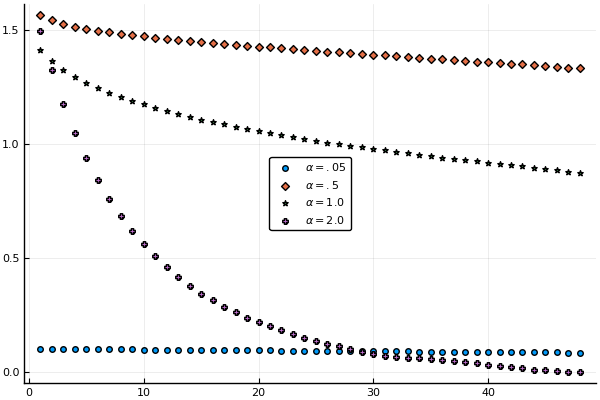
\includegraphics[width=.9\linewidth]{./acf.png}$$


For these different values of \(\alpha\), we plot the histogram and the
pdf of the distribution. As we can see, for the very small value of
\(\alpha\), the distribution is stuck in the first mode of the distribution,
and the rest of the support remains unexplored, even after 50000
steps, and a burnout period of 10000.

For the slightly larger \(\alpha = .5\), we see that most of the distribution
is explored, but the starting point of \(0.0\) is still overstated, even
after 50000 steps, and the far side of the distribution is less
explored. This indicates that the distribution still has not reached
the steady state despite many draws. The same effect is mirrored in
\(\alpha= 1.0\), indicating that this may be simply caused by noise.

For \(\alpha = 2.0\), the histogram almost exactly matches the pdf of the
distribution, indicating that good mixing has been achieved. 

\begin{figure}[H]
\centering
\begin{minipage}{.5\textwidth}
  \centering
  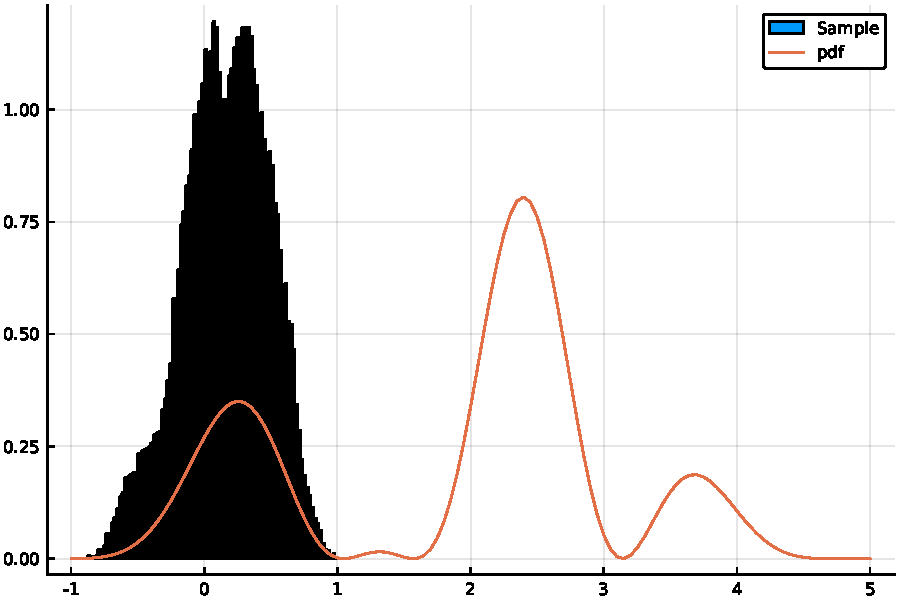
\includegraphics[width=.8\linewidth]{pdf05.pdf}
  \captionof{figure}{$\alpha = .05$}
  \label{fig:test3}
\end{minipage}%
\begin{minipage}{.5\textwidth}
  \centering
  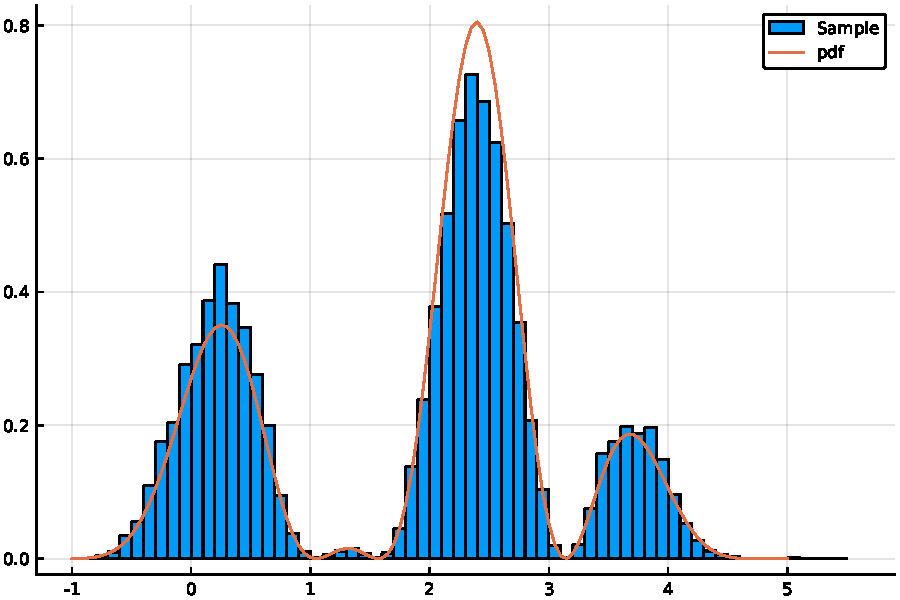
\includegraphics[width=.8\linewidth]{pdf5.pdf}
  \captionof{figure}{$\alpha = .5$}
  \label{fig:test4}
\end{minipage}
\end{figure}

\begin{figure}[H]
\centering
\begin{minipage}{.5\textwidth}
  \centering
  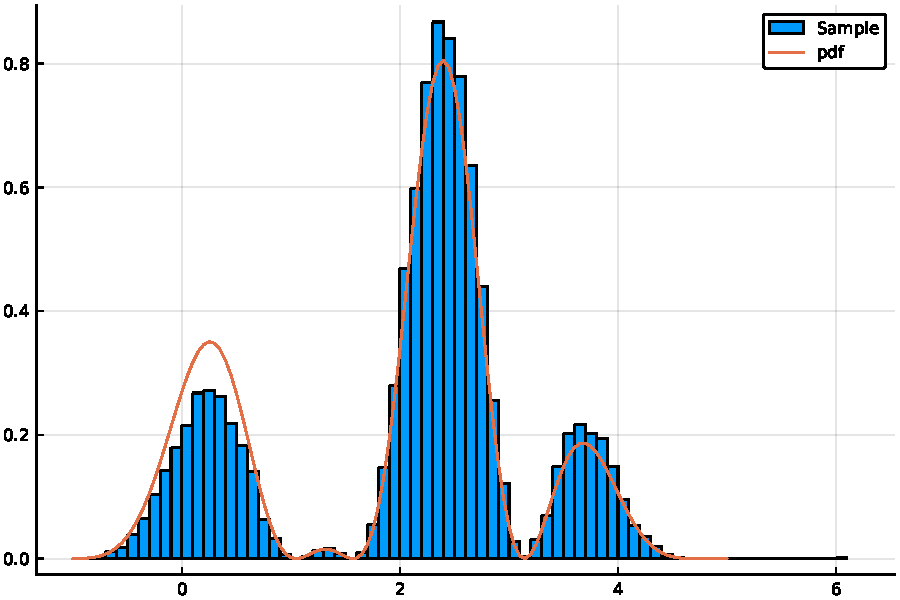
\includegraphics[width=.8\linewidth]{pdf1.pdf}
  \captionof{figure}{$\alpha = 1.0$}
  \label{fig:test3}
\end{minipage}%
\begin{minipage}{.5\textwidth}
  \centering
  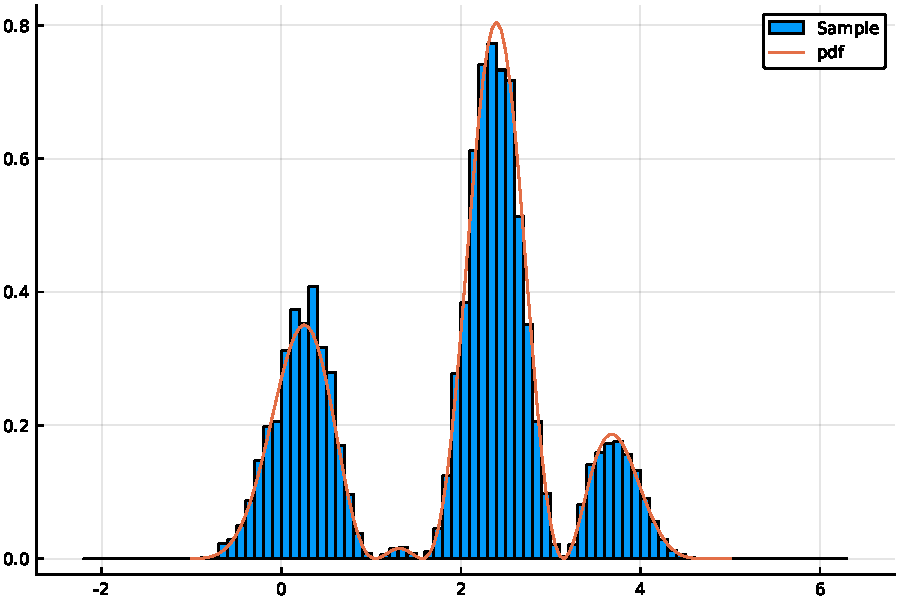
\includegraphics[width=.8\linewidth]{pdf2.pdf}
  \captionof{figure}{$\alpha = 2.0$}
  \label{fig:test4}
\end{minipage}
\end{figure}


\section{Question 4}
\label{sec:org667b640}
\subsection{a}
\label{sec:orgf102039}
Let $\sigma_b^{-2} \sim \Gamma(\alpha_b, \beta_b)$ and $\sigma_{\epsilon}^{-2} \sim \Gamma( \alpha_{\epsilon}, \beta_{\epsilon})$.
$\beta \sim \normal( \mu, \Sigma)$. Note that $\mu$ is a vector with 4 elements, and
that $\Sigma$ is a $4 \times 4$ matrix. This means that there are $24$
hyper-parameters. 

\subsection{b}
\label{sec:orgd42d3c7}
Conditioned on $X_i, \beta, W_i, b_i, \epsilon_i$,
\begin{align*}
  \epsilon_i &\sim \normal( 0, \sigma_{\epsilon}^{2}I)\\
  b_i &\sim \normal( 0, \sigma_{b}^{2})\\
  W_ib_i &\sim \normal( \vec{0}, W_i \sigma_{b}^{2} W_i' )
\end{align*}

$X_i \beta$ is fixed and non-random. The sum of these three must be
normal, where the expected value is the sum of the expected values,
and the variance is given by the sum of the variances.

\begin{equation}
  y_i \sim \normal\left( X_i \beta, \sigma_{\epsilon}^2 I + W_i \sigma_b^2 W_i' \right)
\end{equation}

The Posterior distribution is given by the prior times the likelihood
divided by the normalizing constant.

We may note that $\beta,\sigma_b^{-2}, \sigma_{\epsilon}^{-2}$ are all independent of each
other, so the prior distribution will simply be the product of their
densities.

Therefore the prior density is given by:
\begin{equation}
  f_{\mathcal{N}}(\vec{\mu}, \Sigma) f_{\Gamma}(\alpha_b, \beta_b) f_{\Gamma}(\alpha_{\epsilon}, \beta_{\epsilon})
\end{equation}


The posterior distribution is this prior multiplied by the likelihood
of the normal distribution of $y_i$ given above.

\begin{minted}[frame=lines,fontsize=\scriptsize,xleftmargin=\parindent,linenos,mathescape,breaklines=true,stripnl=true,firstnumber=last]{julia}

# Let $\sigma_b^{-2} \sim \Gamma(\alpha_b, \beta_b)$
# $\sigma_{\epsilon}^{-2} \sim \Gamma( \alpha_{\epsilon}, \beta_{\epsilon})$.
# $\beta \sim \normal( \mu, \Sigma)$


# $y_i \sim \normal\left( X_i \beta, \sigma_{\epsilon}^2 I + W_i \sigma_b^2 W_i' \right)$

data = DataFrame(load("pset1q4.csv"))
N = size(data)[1]

X = Vector{Matrix}(undef,N)
W = Vector{Vector}(undef,N)
Y = Vector{Vector}(undef,N)
for i in 1:N
    X[i] = [data[i,:x11] data[i,:x12] data[i,:x13] data[i,:x14];
            data[i,:x21] data[i,:x22] data[i,:x23] data[i,:x24]]
    W[i] = [data[i,:w1], data[i,:w2]]
    Y[i] = [data[i,:y1], data[i,:y2]]
end


function EvaluateLikelihood( Y::Vector{Vector}, X::Vector{Matrix}, W::Vector{Vector}, β::Vector{Float64}, σe²::Float64, σb²::Float64)
    #Note that the likelihood function of a mutlivariate normal is:
    # $\frac{1}{\sqrt{2 \pi \vert \Sigma \vert}} exp ( -.5 (x - \mu)' \Sigma^{-1} (x-\mu))$

    #Because of numerical concerns we will exponentiate the sum of the logs
    likelihood = (N/2.0)*log(2*pi)
    for i in 1:N
        μ = X[i]*β
        Σ = σe²*I  + σb²*W[i]*W[i]'

        #Sigma is positive definite, so we should invert it using the
        #cholesky decomposition, especially as numerical concerns loom
        F = cholesky(Hermitian(Σ))
        invSigma = (F.U \ (F.L \ I))

        likelihood += -.5*log( det(Σ)) - .5*(Y[i]-μ)'*invSigma*(Y[i]-μ)
    end
    #likelihood = exp(likelihood)
    return likelihood
end

function EvaluatePriors( αe::Float64, αb::Float64, βe::Float64, βb::Float64, μ::Vector{Float64}, Σ::Matrix{Float64}, betaVal::Vector{Float64}, sigmaEVal::Float64, sigmaBVal::Float64 )
    betaPrior = pdf( MvNormal( μ, Σ), betaVal)
    sigmaEPrior = pdf( Gamma( αe, βe), sigmaEVal)
    sigmaBPrior = pdf( Gamma( αe, βe), sigmaBVal)
    #return exp( log(betaPrior) + log( sigmaEPrior) + log( sigmaBPrior))
    return log(betaPrior) + log( sigmaEPrior) + log( sigmaBPrior)
end

function pBeta(β::Vector{Float64}, σe²::Float64, σb²::Float64, Y::Vector{Vector}, X::Vector{Matrix}, W::Vector{Vector}, αe::Float64, αb::Float64, βe::Float64, βb::Float64, μ::Vector{Float64}, Σ::Matrix{Float64} )
    return exp( EvaluateLikelihood(Y,X,W,β,σe², σb²) +EvaluatePriors( αe, αb, βb, βb, μ, Σ, β, σe², σb²) )
end

function qBeta( β, βCond::Vector{Float64}, ::Nothing )
    return 1.0#0.00390625 #1 / 256
end

function qBetaSim( βCond::Vector{Float64}, ::Nothing)
    return [rand(Uniform(βCond[1]-.5, βCond[1]+.5),1)[1],
            rand(Uniform(βCond[2]-.5, βCond[2]+.5),1)[1],
            rand(Uniform(βCond[3]-.5, βCond[3]+.5),1)[1],
            rand(Uniform(βCond[4]-.5, βCond[4]+.5),1)[1]]
end

#This is the same as pBeta except we have reordered the first 3 arguments
function pSigmaE(σe²::Float64,β::Vector{Float64},  σb²::Float64, Y::Vector{Vector}, X::Vector{Matrix}, W::Vector{Vector}, αe::Float64, αb::Float64, βe::Float64, βb::Float64, μ::Vector{Float64}, Σ::Matrix{Float64} )
    return exp( EvaluateLikelihood(Y,X,W,β,σe², σb²) +EvaluatePriors( αe, αb, βb, βb, μ, Σ, β, σe², σb²) )
end


#This is the same as pBeta except we have reordered the first 3 arguments
function pSigmaB(σb²::Float64,β::Vector{Float64},  σe²::Float64, Y::Vector{Vector}, X::Vector{Matrix}, W::Vector{Vector}, αe::Float64, αb::Float64, βe::Float64, βb::Float64, μ::Vector{Float64}, Σ::Matrix{Float64} )
    return exp( EvaluateLikelihood(Y,X,W,β,σe², σb²) +EvaluatePriors( αe, αb, βb, βb, μ, Σ, β, σe², σb²) )
end

function qSigma( σ::Float64, σCond::Float64, ::Nothing)
    return pdf(Uniform(max(σCond - 2.0,0), σCond + 2.0),σ)
end

function qSigmaSim( σCond::Float64, ::Nothing)
    return rand(Uniform(max(σCond - 2.0,0),σCond + 2.0),1)[1]
end

\end{minted}

\begin{minted}[frame=lines,fontsize=\scriptsize,xleftmargin=\parindent,linenos,mathescape,breaklines=true,stripnl=true,firstnumber=last]{julia}


priorAe = 1.0
priorBe = 1.0
priorAb = 1.0
priorBb = 1.0
priorMu = [1.0,1.0,1.0,1.0]
priorSigma = [1.0 0 0 0; 0 1.0 0 0; 0 0 1.0 0; 0 0 0 1.0]

initBeta = [0,0,0,0]
initSigmaE = 2.0
initSigmaB = 2.0

M = 20000
U = rand(Uniform(), M)

β = Vector{Vector{Float64}}(undef,M)
β[1] = initBeta
σE = Vector{Float64}(undef,M)
σE[1] = initSigmaE
σB = Vector{Float64}(undef,M)
σB[1] = initSigmaB


#This is my implementation of the Gibbs Sampler.
for i in 2:M
    #Simulate β:
    β[i] = Metropolis( β[i-1], 1, pBeta, qBeta, qBetaSim, [σE[i-1],σB[i-1], Y, X, W, priorAe, priorAb, priorBe, priorBb, priorMu,priorSigma], [nothing])[2]
    σE[i] = Metropolis( σE[i-1], 1, pSigmaE, qSigma, qSigmaSim, [β[i],σB[i-1], Y, X, W, priorAe, priorAb, priorBe, priorBb, priorMu,priorSigma], [nothing])[2]
    σB[i] = Metropolis( σB[i-1], 1, pSigmaB, qSigma, qSigmaSim, [β[i],σE[i], Y, X, W, priorAe, priorAb, priorBe, priorBb, priorMu,priorSigma], [nothing])[2]
    if( i % 1000 == 0)
        println(i)
    end
end


betaOne = Vector{Float64}(undef,M)
betaTwo = Vector{Float64}(undef,M)
betaThree = Vector{Float64}(undef,M)
betaFour = Vector{Float64}(undef,M)
for i in 1:M
    betaOne[i] = β[i][1]
    betaTwo[i] = β[i][2]
    betaThree[i] = β[i][3]
    betaFour[i] = β[i][4]
end

# histogram(betaOne[2000:end], normalize = true)

histogram(σB[2000:end], normalize=true, label = "\$\\sigma_{b}\$")
savefig( "sigmaB.pdf" )
histogram(σE[2000:end], normalize=true, label = "\$\\sigma_{\\epsilon}\$")
savefig( "sigmaE.pdf" )


p1 = histogram(betaOne[2000:end], normalize=true, title = "\$\\beta_{1}\$")
p2 = histogram(betaTwo[2000:end], normalize=true, title = "\$\\beta_{2}\$")
p3 = histogram(betaThree[2000:end], normalize=true, title = "\$\\beta_{3}\$")
p4 = histogram(betaFour[2000:end], normalize=true, title = "\$\\beta_{4}\$")
plot(p1,p2,p3,p4,layout=(2,2), legend=false)
savefig("betaHist.png" )
\end{minted}

\begin{center}
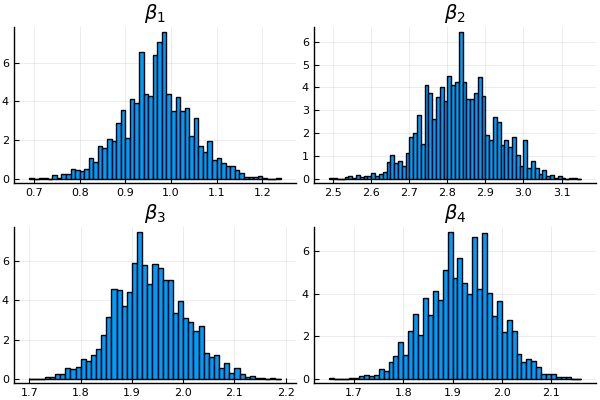
\includegraphics[width=.9\linewidth]{./betaHist.png}
\end{center}

As we can see, the \(\beta\) distribution remains relatively noisy on the
marginal pdfs, but is still dispersed. This data is sampled after
20000 iterations, with a burn-in period of 2000. There is a relatively
low acceptance rate for the betas of only 10\%, but as the likelihood
function suffered such numerical problems, this was the best result
that I could muster. For a better chosen \(q\) function, it is likely
that better mixing could be achieved for the \(\beta\) distribution. The
priors used were \(\beta = 0\), so it is clear that the distribution has
moved away from the priors, and has learned from the likelihood
function.

Since the marginal distributions do not show the variance structure,
it is difficult to say more about the multivariate normal that is
sampled from the Gibbs-sampler simply by examining the histogram of the
values of each of its marginals. However, we may notice that there is
quite low auto-covariance within each of the marginal distributions.

\begin{center}
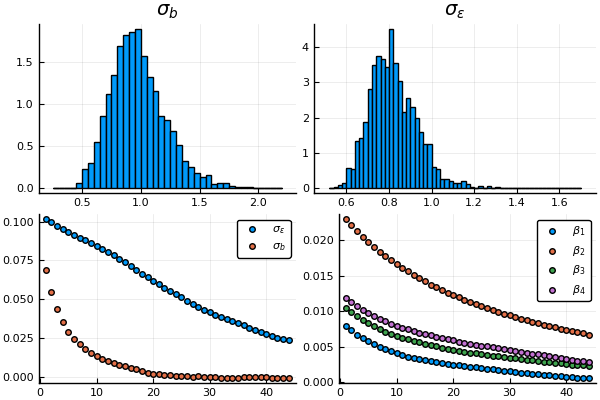
\includegraphics[width=.9\linewidth]{./CorrelationSigma.pdf}
\end{center}

The distribution for the univariate \(\sigma_b\) is quite
nicely uni-modal. It is clear that the distribution has reached its
stationary distribution and is mixing relatively well by the
relatively noise-less histogram. The acceptance rate of this
distribution is 15\%, which is relatively low, but still enough to
ensure that we are sampling from the stationary distribution after
20000 iterations. There is extremely low auto-covariance between the
different sigma values, indicating that there is a decent mixture from
the distribution. The prior values that were chosen were $2.0$, which
appears very little in the distribution, so we can believe that they
are uninformative for the actual distribution of the data.

While this distribution is not quite as clean as the distribution of
\(\sigma_b\), $\sigma_{\epsilon}$ is still uni-modal, and appears to be at the stationary
distribution of the variance. While the prior for this variance was
\(2.0\), the distribution has settled itself at a lower value,
indicating that it has moved away from the prior. The auto-covariance
is relatively low, but does not fall linearly (from the log axis) as
the distribution of $\sigma_b$ does. There is however a higher acceptance
rate of $20\%$, which may explain why there is a higher
auto-covariance between the different samples. 


\end{document}